%%%%%%%%%%%%%%%%%%%%%%%%%%%%%%%%%%%%%%%%%
% University/School Laboratory Report
% LaTeX Template
% Version 3.1 (25/3/14)
%
% This template has been downloaded from:
% http://www.LaTeXTemplates.com
%
% Original author:
% Linux and Unix Users Group at Virginia Tech Wiki 
% (https://vtluug.org/wiki/Example_LaTeX_chem_lab_report)
%
% License:
% CC BY-NC-SA 3.0 (http://creativecommons.org/licenses/by-nc-sa/3.0/)
%
%%%%%%%%%%%%%%%%%%%%%%%%%%%%%file:///home/giulio/Documents/MHPC/Foundations_of_HPC_2020/Assignement1/report/tex/sample.bib
%%%%%%%%%%%%

%----------------------------------------------------------------------------------------
%	PACKAGES AND DOCUMENT CONFIGURATIONS
%----------------------------------------------------------------------------------------

\documentclass{article}

\usepackage{geometry}
 \geometry{
 a4paper,
 left=15mm,
 right=15mm,
 bottom = 25mm,
 }


\usepackage{graphicx} % Required for the inclusion of images
\graphicspath{ {./plots/} }

\usepackage{natbib} % Required to change bibliography style to APA
\usepackage{amsmath} % Required for some math elements 

\setlength{\parskip}{\baselineskip}%
\setlength{\parindent}{0pt}% % Removes all indentation from paragraphs

\renewcommand{\labelenumi}{\alph{enumi}.} % Make numbering in the enumerate environment by letter rather than number (e.g. section 6)

%\usepackage{times} % Uncomment to use the Times New Roman font


%custom packages
\usepackage{subcaption}
\usepackage{float}

\setlength{\abovecaptionskip}{5pt}



%----------------------------------------------------------------------------------------
%	DOCUMENT INFORMATION
%----------------------------------------------------------------------------------------

\title{Report on Assignment 1 \\ Foundations of HPC} % Title

\author{\textsc{Giulio Dondi}} % Author name

\date{\today} % Date for the report

\begin{document}

\maketitle % Insert the title, author and date


% If you wish to include an abstract, uncomment the lines below
% \begin{abstract}
% Abstract text
% \end{abstract}

\tableofcontents




%----------------------------------------------------------------------------------------
%	SECTION 1
%----------------------------------------------------------------------------------------


\section{Section 1 - Theoretical Model}

In this section we consider computer algorithms for the addition of $N$ given numbers, and build models to predict their run-times. The simplest solution to the problem is a serial algorithm for on a single processor, executing the following steps: 
\begin{itemize}
\item Read the list of $N$ numbers to be added, incurring a time delay $T_{read}$ which we treat as independent of $N$.
\item Perform $\left( N - 1 \right)$ addition operations, which takes a time $\left( N - 1 \right)T_{calc}$
\end{itemize}

The serial runtime is then:
\begin{equation}
T_s \left( N \right) = T_{read} +  \left( N -1 \right)T_{calc}
\end{equation}

If we have $c$ processors at our disposal the algorithm can be parallelised, as the numbers to be added can be distributed among the processors which work simultaneously. The need to transfer data among the processors requires a communication network and is bound to add time penalties.\\
A na\"ive parallel algorithm on $c$ processors entails the folllowing steps:

\begin{itemize}
\item The master process reads the list of $N$ numbers to be added, incurring a time delay $t_{read}$ which we treat as independent of $N$.
\item The master process distributes the numbers evenly to the $\left( c - 1 \right) $ slave processors. The communication time delay is $\left( c - 1\right) T_{comm}$
\item Each processor now holds $N/c$ numbers and performs $\left( N/c - 1 \right)$ addition operations, which takes a time $\left( c - 1 \right)T_{calc}$
\item Each slave processor sends its partial result back to the master processor. The master processor can only receive one message at a time, therefore the time taken for all communications is $\left( c - 1\right) T_{comm}$
\item The master processor adds up the partial results in a time  $\left( c - 1\right) T_{calc}$
\end{itemize}

The runtime of this parallel algorithm is then:

\begin{equation}
T_p \left( N, c \right) = T_{read} + 2\left( c - 1 \right)T_{comm}  +  \left( N/c + c - 2 \right)T_{calc}
\end{equation}

The two algorithms can be compared by computing the \textit{Speedup} $S = \frac{T_s}{T_p\left( c \right)}$ as a function of the number of processors employed. The example values used are listed in table \ref{th_table}. Speedup curves were computed against $c$ varying between 1 and 100 for several values of the problem size $N$, and are displayed in figure \ref{th_speedup_1}.

\begin{center}
\label{th_table}
 \begin{tabular}{|c | c | c | c|} 
 \hline
 $T_{comm}$ & $T_{calc}$ & $T_{read}$ \\ 
 \hline
 $1 \times 10^{-6} $ & $2 \times 10^{-6}$ & $1 \times 10^{-4}$\\ 
 \hline
\end{tabular}
\end{center}







\begin{figure}[H]
  \begin{subfigure}[b]{0.5\textwidth}
    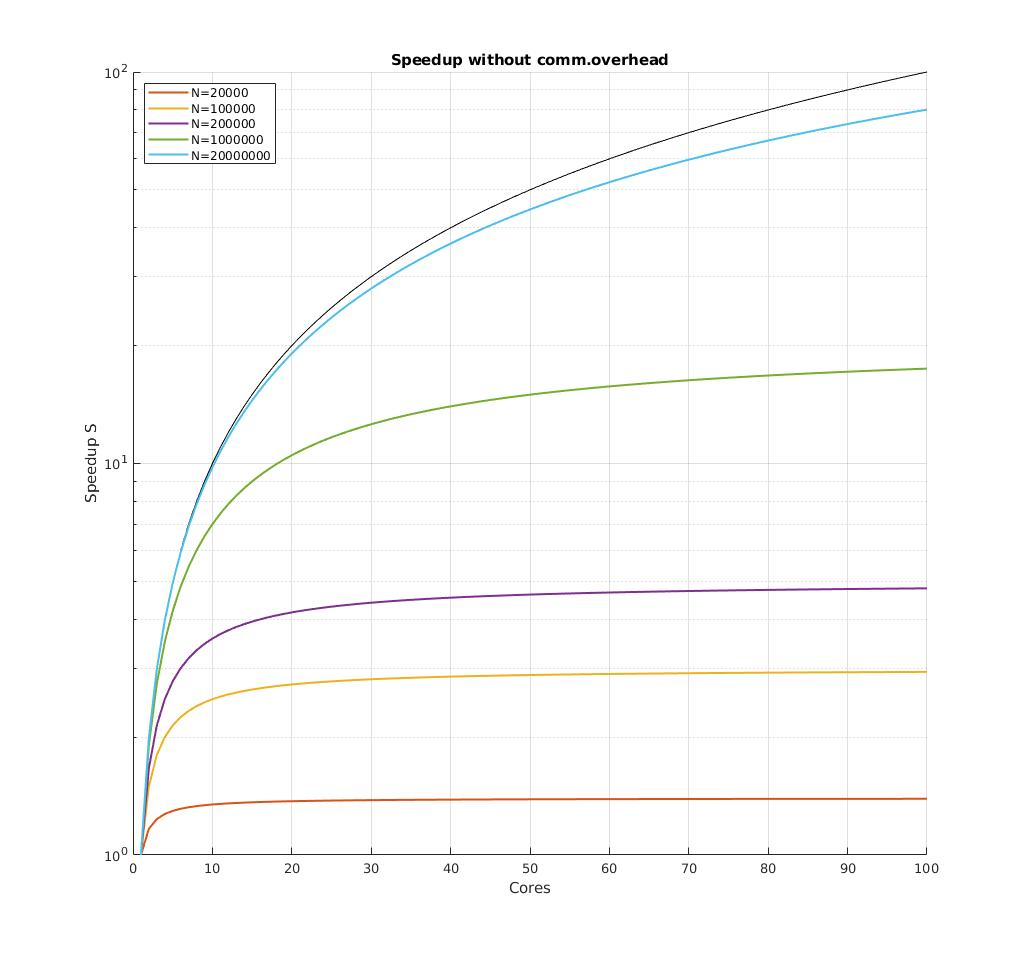
\includegraphics[width=1.2\textwidth]{th_scaling_0}
    \caption{No communication overhead}
    \label{th_speedup_1a}
  \end{subfigure}
  %
  \begin{subfigure}[b]{0.5\textwidth}
    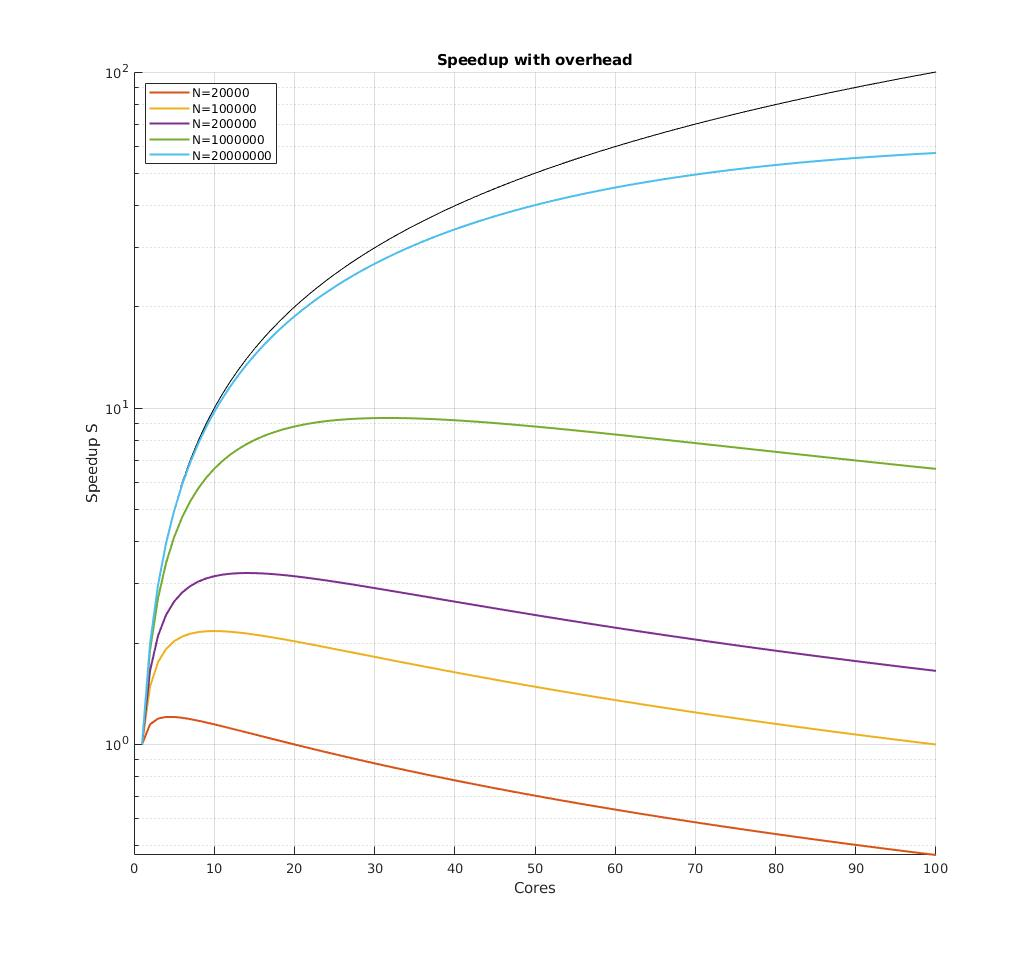
\includegraphics[width=1.2\textwidth]{th_scaling_1}
    \caption{with communication overhead}
    \label{th_speedup_1b}
  \end{subfigure}
  \caption{Semilog. plots of the Speedup curves for the na\"ive parallel algorithm for various values of $N$, setting $T_{comm}=0$ for the left graph and using the value of table \ref{th_table} on the right. The black curve represents ideal speedup.}
  \label{th_speedup_1}
\end{figure}



Ideal speedup entails that a problem of size $N$ over $c$ processors is $c$ times faster, although this is impossible to achieve practically for two main reasons.\\
First, only a fracton of the work may be split among the processors, while the \textit{serial fraction} $s$ remains whole. \textit{Amdahl's law} states that the speedup is limited by the serial fraction, more precisely that the asymptotic speedup fir infinite processors is $S=1/s$.\\
The serial part of the algorithm is represented by $T_{read}$ in our case. Since the reading phase takes a time $T_{read}$ regardless of problem size by assumption and the rest depends linearly on $N$, the serial fraction depends inversely on $N$. Amdahl's law then predicts that the asymptotic speedup increases with $N$, which can be clearly seen in figure \ref{th_speedup_1a}.\\
The second factor is the communication overhead, which is exacerbated by the fact that all communications pass through the master process and are thus serialized. This adds a serial contribution to the algorithm which is independent of $N$ but grows with $c$. Figure \ref{th_speedup_1b} shows the effect of the overhead: the speedup is impaired more and more with increasing $c$ until a maximum value is reached, when the overhead causes a net slowdown of performance. This effect is less pronounced ad $N$ increases, since this overhead becomes less important compared with the parallel fraction. For the same reason, as $N$ increases, the maximum speedup is reached at higher values of $c$, for the largest value of $N$ studied the maximum is in fact not reached in the given range of processor values.

\par
To improve the algorithm it is natural to operate on the communication part, altering the workflow so that at least part of the communication may be parallelised.\\
The new workflow is as follows:


\begin{itemize}
\item The algorithm is identical to the previous parallel one up until the $c$ partial sums are computed
\item Instead of sending all the results to the master processor, the processors are divided in pairs where one sends its result to the other, which computes a new partial sum. All messages can be sent simultaneously as all processors either send or receive just one message, so this step lasts just $\left( T_{calc} + T_{comm} \right)$
\item The previous step is repeated for the $c/2$ processors holding the new partial sums, and so on until just the master processor is left in possession of the final sum
\end{itemize}

IF $c$ is a power of $2$ i.e. $c=2^d$, then it is trivial to see that the number of communication steps is $d=log_2 c$, and therefore the total communication time is $\left( T_{calc} + T_{comm} \right)log_2 c$. Even if $c$ is a generic number $2^d < c < 2^{d+1}$ the number of steps is still $c$: in this case we can separate the processors in a group of $2^d$ and split the remaining processors in groups of $2^m$ where $m$ is some integer strictly smaller than $d$ itself. These smaller groups would compute their partial sum using the same logic in $m$ steps in parallel with the larger group and then wait for it to finish, upon which all the partial sums would be communicated and added serially.\\
The time penalty of this approach is, in general:
\begin{equation}
\left( T_{calc} + T_{comm} \right)\times \left( log_2 c + x - 1\right) \sim \left( T_{calc} + T_{comm} \right)\times  log_2 c
\end{equation}
where $x$ is the number of power-of-two groups that compose $c$, which may be computed by converting $c$ in base-2 representation, treating the result as decimal and adding up its digits. For the sake of simplicity, we neglect this $x-1$ term in the following since the qualitative characteristics of the speedup curves are captured nonetheless.

The revised algorithm has thus a runtime of:

\begin{equation}
T_p ^\prime \left( N, c \right) = T_{read} + \left( c - 1 \right)T_{comm}  +  \left( N/c -1 \right)T_{calc} + \left( T_{calc} + T_{comm} \right) log_2 c
\end{equation}

In figure \ref{th_speedup_2} the speedup curves for this new algorithm are shown, calculated for the same range of $c$, the same values of $N$ and using the same parameters of table \ref{th_table}. \\
It is clear from figure \ref{th_speedup_2a} that the new message-passing algorithm reduces the impact of the communication overhead, but does not eliminate it completely. The trends set by Amdahl's law with overheead are thus preserved. As evidenced in figure \ref{th_speedup_2b}, the improvement is proportional to the problem size $N$ and tends to taper off around some value of $c$, this point depends of course on the problem size, so much that the largest value of $N$ studied does not reach it in the set range of $c$.



\begin{figure}[H]
  \begin{subfigure}[h]{0.5\textwidth}
    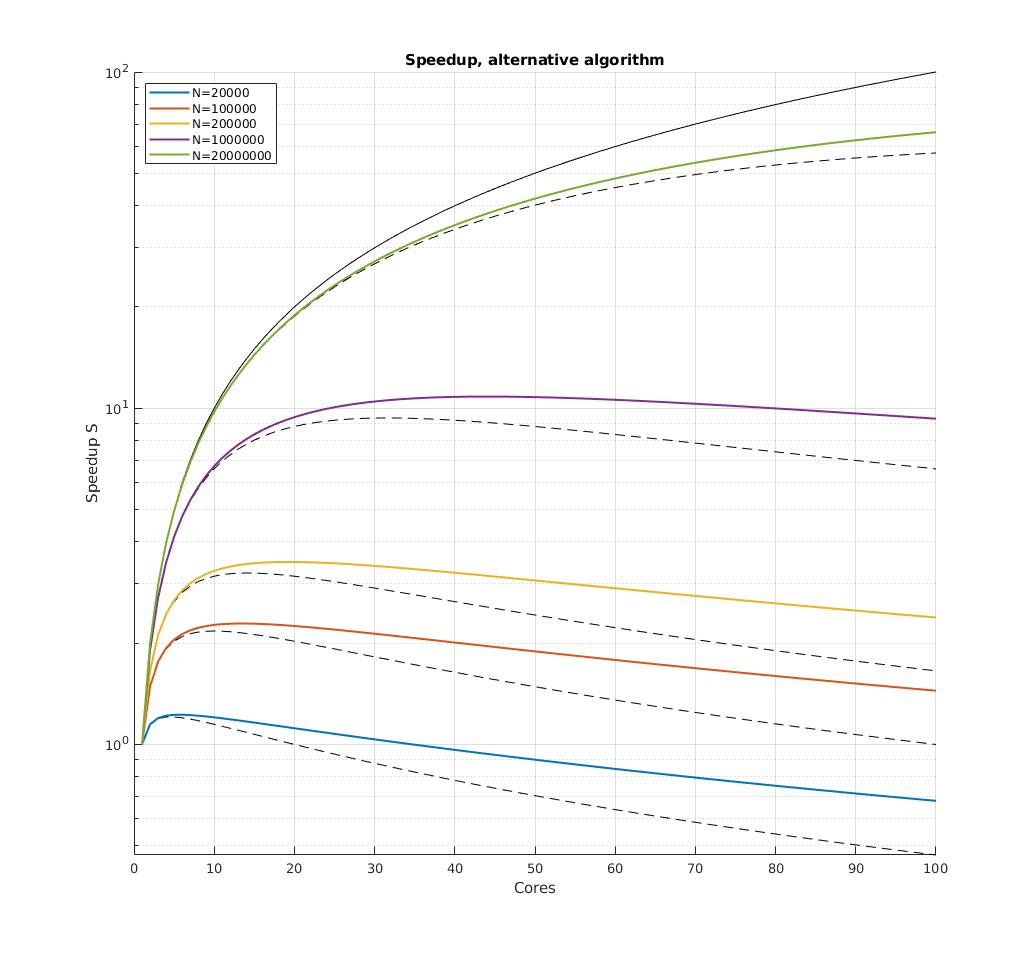
\includegraphics[width=1.1\textwidth]{th_scaling_2}
    \caption{Speedup of improved algorithm}
    \label{th_speedup_2a}
  \end{subfigure}
  %
  \begin{subfigure}[h]{0.5\textwidth}
    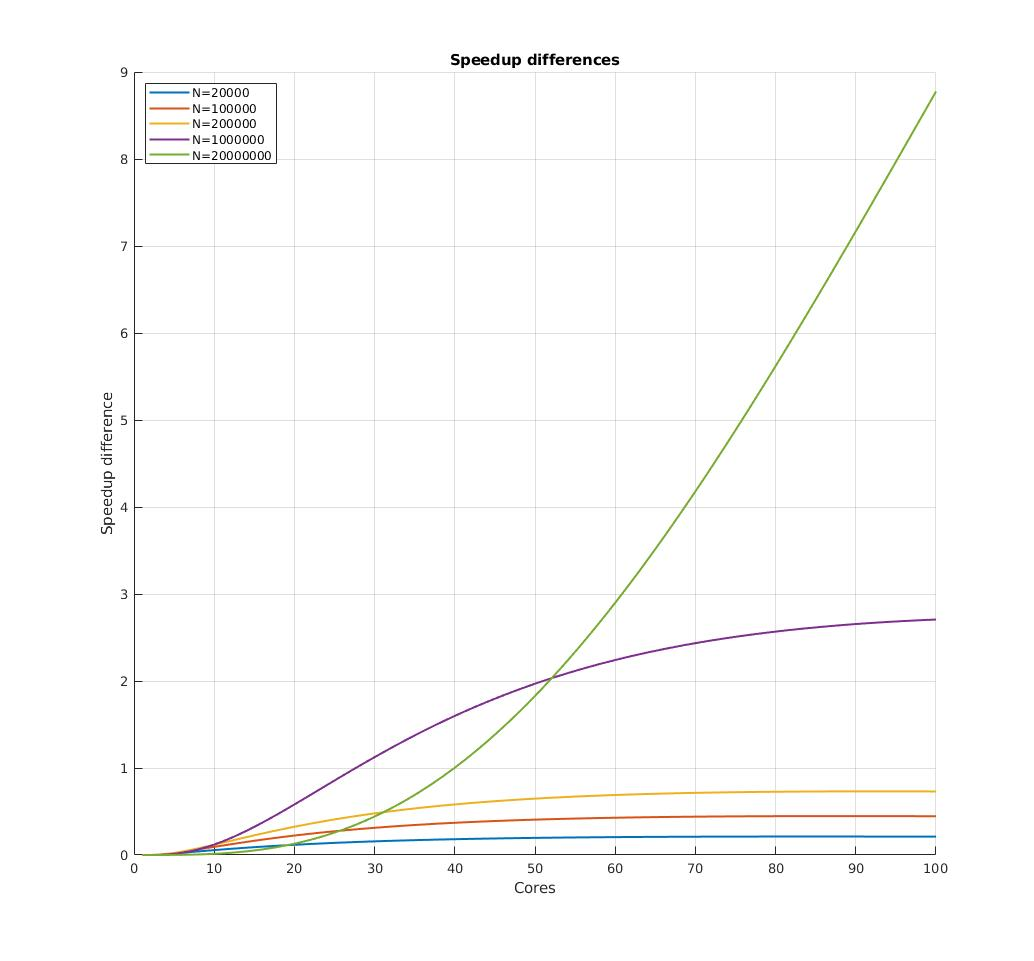
\includegraphics[width=1.1\textwidth]{th_scaling_comp}
    \caption{Speedup difference.}
    \label{th_speedup_2b}
  \end{subfigure}
   \caption{On the left: semi-log. speedup plot of the improved algorithm, where the black dashed lines are the speedup curves of the old algorithm for comparison. On the right: Difference of the speedup curves against $p$ between the two algorithms in linear scale}
   \label{th_speedup_2}
\end{figure}



%----------------------------------------------------------------------------------------
%	SECTION 2
%----------------------------------------------------------------------------------------



\section{Section 2 - MPI program}

In this section the performance of a \verb|C|-language Monte-Carlo algorithm for the calculation of $\pi$ is analysed. The algorithm generates $N$ random points in a square of side 1. A counter $M$ keeps track of the fraction of these points which lie in the circle quadrant centered at the origin, and $\pi$ may be extracted from the relation $M/N = \pi /4$.\\
The number generation can be distributed to $p$ processors, which receive the number $N/p$ of points to generate and communicate the fraction $M_i$ back to the master processor. The fractons are finally summed together and $\pi$ is extracted in the same way. The parallel algorithm uses the \verb|MPI| framework to spawn all processes and communicate between them.
\par 
First, the serial performance of the algorithm was tested for various values of the problem size: $N=\{ 10^8 , 10^9 , 10^{10} , 10^{11} \} $. The runtimes $T_s$ are displayed in figure \ref{serial_scaling}, which displays a clear linear dependency on the problem size.

\begin{minipage}{\linewidth}
\begin{minipage}{0.6\linewidth}
\label{serial_scaling}
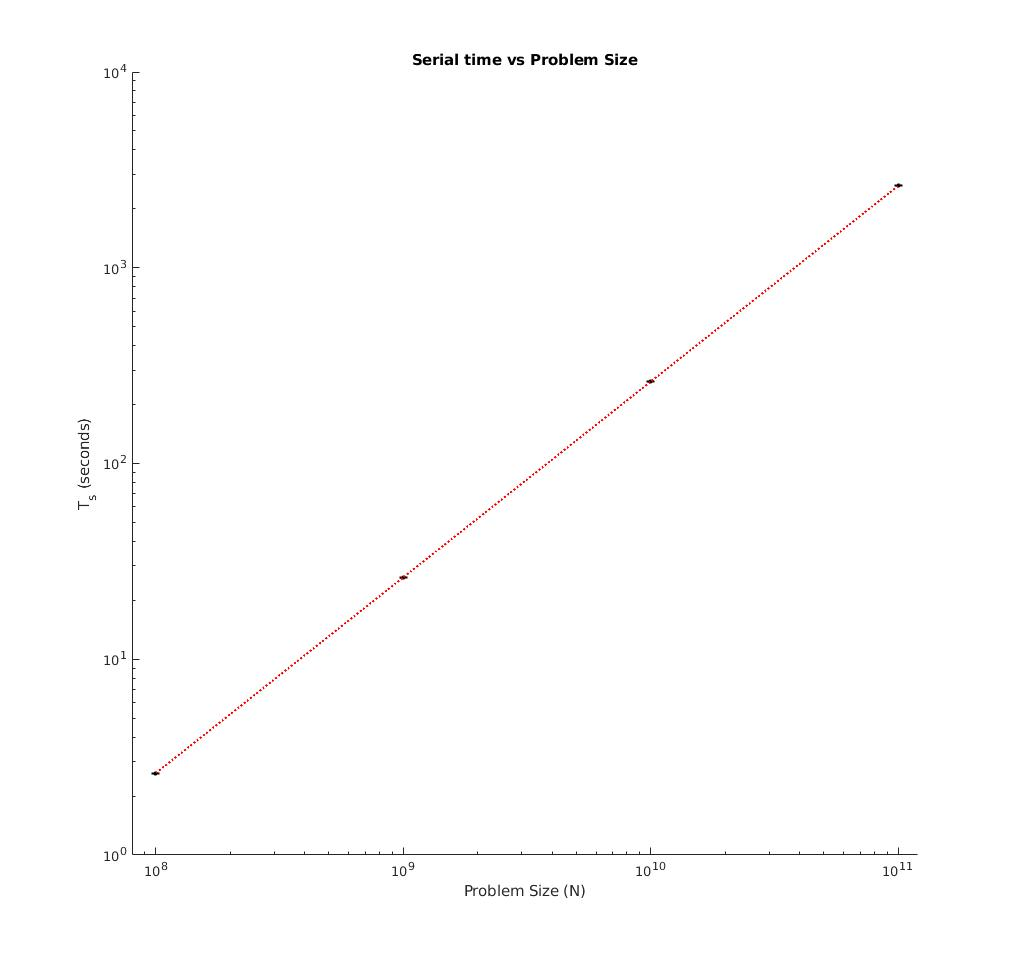
\includegraphics[width=0.8\textwidth]{Serial_times}
\captionof{figure}{Log-log plot of the serial run-times against $N$. }
\end{minipage}
\begin{minipage}{0.4\linewidth}
The linear dependency is expected since the majority of the operations performed belong to the random point geenration section of the algorithm. A simple theoretical model for the serial time was formulated and fitted to the data:

\begin{center}

\begin{equation}
T_s = s + p\times N	
\end{equation}


 \begin{tabular}{|c | c | } 
 \hline
 $s$ & $ 3.368\times 10^{-14}  $  \\ 
 \hline
 $p$ & $ 0.2625\times 10^{-7} $ \\
 \hline
\end{tabular}
\captionof{table}{Serial runtime fit coefficients}
\label{serial_coefs}

\end{center}



The coefficient names reflect the fact that the random-point generation corresponds to the parallel part of the algorithm which will be distributed.

$p$ was chosen as the label for the $N$-term coefficient since the parallel algorithm will distribute this part of the work among the processors, while the independent part $s$ will remain as the serial part.
\end{minipage}

\end{minipage}

Table \ref{serial_frac} reports the "serial fraction" repesented by $s$ for the numbers of $N$ under advisement, showing that indeed the non-parallelisable part of the algorithm is very small.\\
Based on these numbers we will regard the algorithm as "perfectly parallelisable" and neglect the $s$ term, writing $T_s = p \times N$.

\begin{center}
\label{serial_frac}
 \begin{tabular}{|l | c | } 
 \hline
 $N$ & $ s / \left( s + pN \right) $  \\ 
 \hline
 \hline
 $10^{8}$ & $1.283\times 10^{-14}$ \\
 \hline
 $10^{9}$ &  $1.283\times 10^{-15}$\\
 \hline
 $10^{10}$ &  $1.283\times 10^{-16}$\\
 \hline
 $10^{11}$ &  $1.283\times 10^{-17}$\\
 \hline
\end{tabular}
\captionof{table}{"Serial fraction" vs. $N$ }
\end{center}



Next, the performance of the serial algorithm was compared against the parallel algorithm running on a single core, run-times were recorded for all four values of $N$ for both algorithms. A single core means that no work distirbution will occur, but the parallel version of the algorithm will still display the effects of some of the overheads arising from the \verb|MPI| framework, namely those related to initialising MPI and the extra serial steps associated with determining the role (master or slave) that a process ought to play.



\begin{minipage}{\linewidth}
\begin{minipage}{0.6\linewidth}
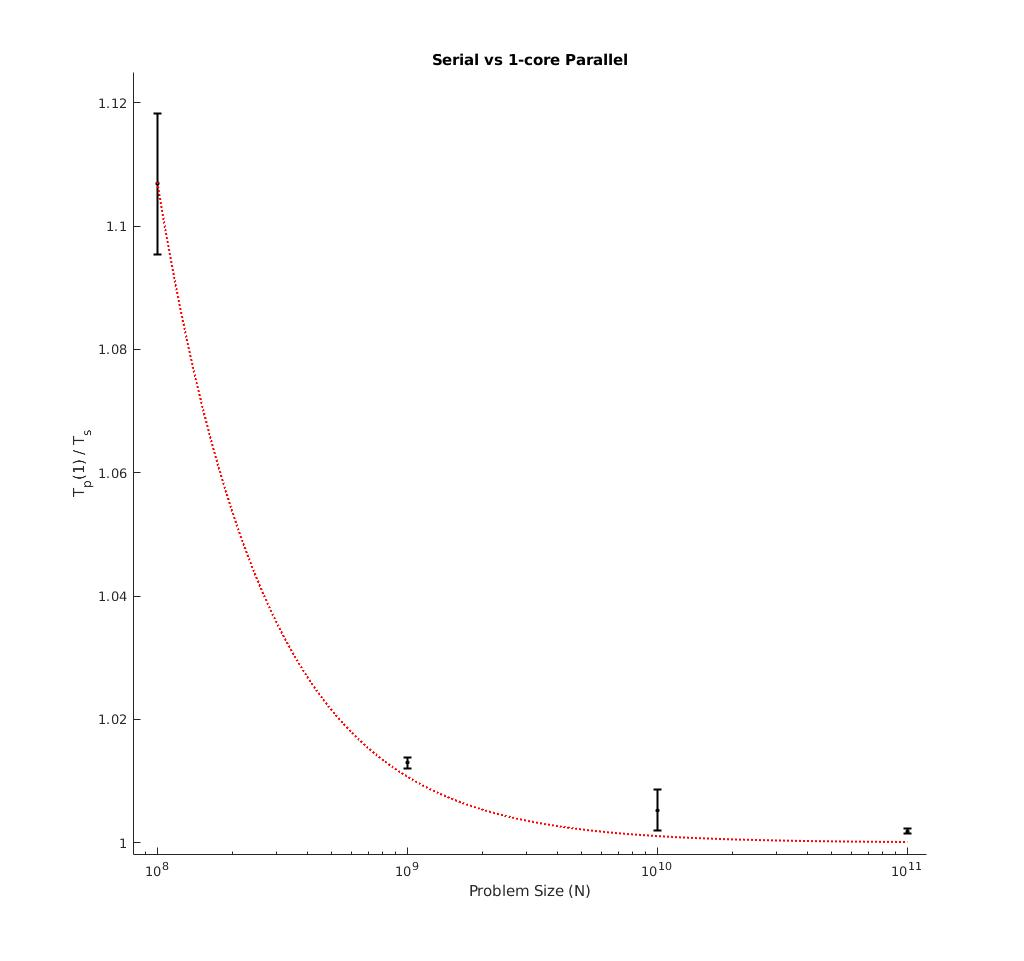
\includegraphics[width=0.8\textwidth]{serial_vs_1core}
\captionof{figure}{Semi-log plot of the ratio $T_p \left( 1 \right) / T_s $ against problem size.}
\label{serial_vs_1core}
\end{minipage}
\begin{minipage}{0.4\linewidth}
Figure \ref{serial_vs_1core} displays the values of the ratio $T_p \left( 1 \right) / T_s $ for all the values of $N$ studied, to determine the magnitude of these overheads in the one-core case. It can be seen that in all four cases the serial algorithm performs better, although the overheads are less important as the problem size grows.\\
A crude model was constructed to fit the data:
\begin{gather*}
\frac{T_p \left( 1 \right) }{T_s} = 1 + a\times\frac{1}{N}	\\
a = 0.10714
\end{gather*}  

This model indicates that since the overhead is a constant time delay it is indeed roughly inversely-proportional to the problem size, although the fit is poorer for large problem sizes.

\end{minipage}

\end{minipage}


These results determined that the "best serial algorithm" that ought to be used to calculate the speedup curves is the non-\verb|MPI| serial one.

\subsection{Strong scaling}

We move on to considering the strong scaling of this problem: the run-times of the parallel algorithm were recorded for varying number of processors: $c=\left\{ 1, 4, 8, 12, \dots , 48 \right\}$ keeping $N$ fixed throughout for all values of the problem size. For each combination of $\left(c,N\right)$ three runs were performed to collect more data. The average runtimes and their error bars are plotted for four values of the problem size $N=\left\{ 10^{8}, 10^{9}, 10^{10}, 10^{11} \right\}$ in Figure \ref{strong_runtimes}.

\begin{figure}[h]
\centering
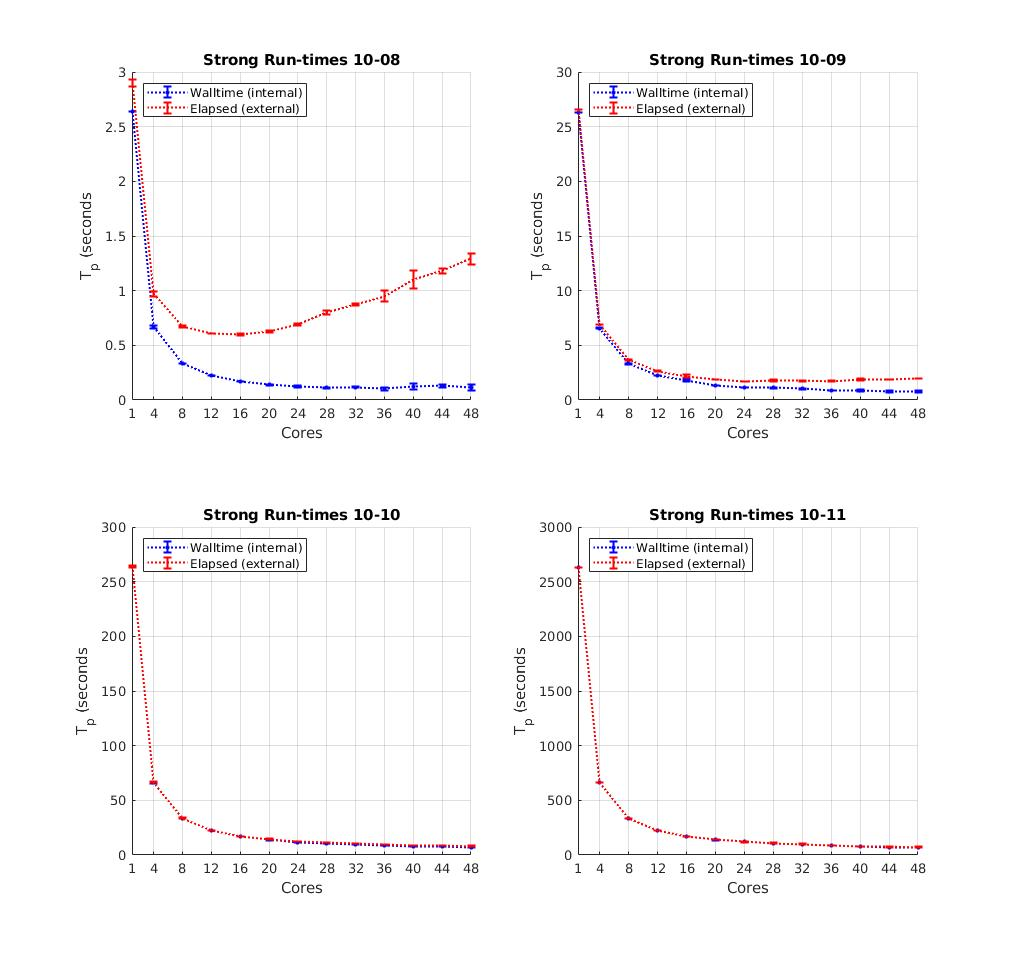
\includegraphics[width=0.85\textwidth]{strong_runtimes}
\caption{Strong-scaling runtimes against the number of processors $c$ for different values of the problem size $N$. Blue curves represent the "walltime" internal to the program, while the red curves use the externally measured run-time}
\label{strong_runtimes}
\end{figure}

Two different measures of run-time were gathered. One is measured externally to the program using the utility \verb|/usr/bin/time|, of all the measurements offered by the utility the "elapsed" time was chosen as it represents the overall real-time interval between program start and program completion. The second one is dubbed "walltime" and is computed internally by each process spawned: The time measurement starts before the start of the random point generation,; slave processes stop measuring once the $M_i$ number has been succesfully sent to the master process, while the master process stops after all messages have been received and the value of $\pi$ has been computed.\\
Strong scaling is defined as $S = T\left( 1 \right) / T_p \left( x \right) $, where $T\left( 1 \right)$ is the best available sequential algorithm, following the previous analysis we will use the purely-serial algorithm in its place. Figure \ref{strong_scaling1} shows the scaling curves for varying $c$ computed using, for kinds of time measurements, the average over the three runs. For the internal "walltime" the largest time value among all the processors was extracted, in all cases the error is obtained as $\left( maxval - minval\right)/2$ over the three runs, combined with the serial time error through propagation.


\par
Let us focus on the behaviour of each panel as $c$ varies.
The blue curves correspond to the internal walltime, and evidently show the presence of overheads dependent on $c$ which cause the speedup to be less than perfect as $c$ increases. Given the way these times are computed they exclude the overhead associated with the initialisation of the MPI framework and the processor ranking while, on the other hand, include the communication overhead given by the message-passing between processors.\\
The communication function used by the slave processors to send their output to the master is \verb|MPI_Ssend()| (\textit{	synchronous send}), which will store the data to be sent in a buffer, handshake with the receiving process and return only when the internal buffer is empty of all the outgoing data and ready for re-use \textit{and} when the receiving process had acknowledged that it has started receiving the bits of the message in its own buffer.  This is to guarantee that the  algorithm flow between the slave and master processor is synchronised at the message-passing instructions, as the message may have left the sender some time before it is being recorded into the receiving buffer. On the receiving end, the master process loops over the slave processors and calls the \verb|MPI_Recv| routine for each of them, which will wait for the sending processor to be ready to send and move on only when the communication had been succesful. For these reasons the communication is serialised and thus the overhead it brings along is proportional to $\left(c - 1\right)$, the number of communications to be performed.


\begin{figure}[h]
\centering
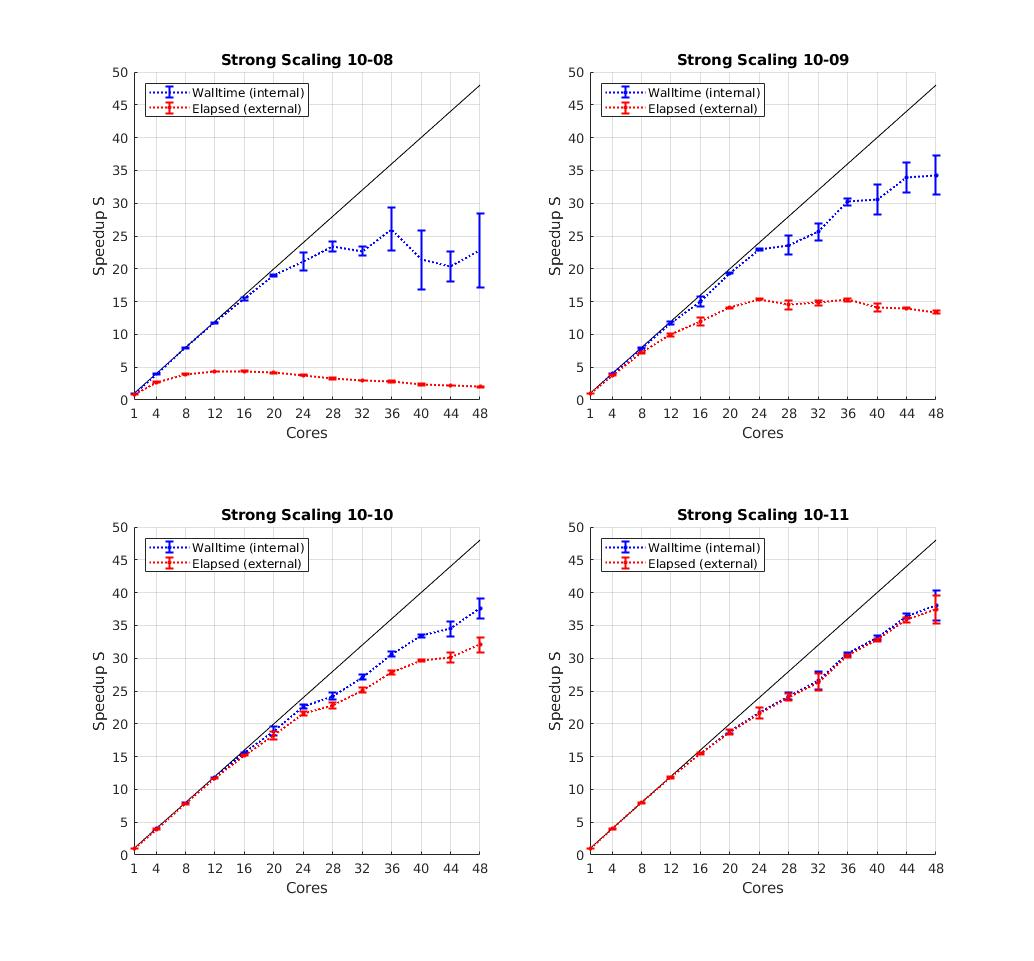
\includegraphics[width=0.85\textwidth]{strong_scaling1}
\caption{ Speedup curves for the parallel algorithm against the number of processors $c$ for different values of the problem size $N$. Blue curves represent the "walltime" internal to the program, while the red curves use the externally measured run-time. The black line represents ideal speedup.}
\label{strong_scaling1}
\end{figure}

\par
Let us focus on the relationship between this overhead and the problem size $N$ by comparing the blue lines across all four panels or, equivalently, looking at the left panel of figure \ref{strong_scaling2}. Ad $N$ grows the curves tend towards an asymptotic state, indicating that the impact of the communication overhead shrinks as the problem grows in size. However, if this overhead were completely independent of $N$ we would expect the asymptotic limit to actually be the ideal speedup line. This does not appear to be the case, and Amdahl's law would suggest that the overhead also carries some dependency on $N$ so that the run-time fraction it represents is constant and constitutes a serial fraction.
The red curves are computed using the external time therefore include both the communication overhead and the initialisation overhead. This last one is also serialised, as the processes are spawned one after the other, this time the dependency is linear with $c$ as all processes require the initialisation of the \verb|MPI| framework. The red curves show that this overhead is much more taxing on the speedup for the smaller values of $N$, while being brely perceptible for the largest value of $N$. It still holds true that the impact of the overheads depends on how big of a percentage of each processor's runtime they represent. The right panel of figure \ref{strong_scaling2} shows how the overheads become smaller and smaller relative to a growing problem size.

\begin{center}
\begin{figure}[h]
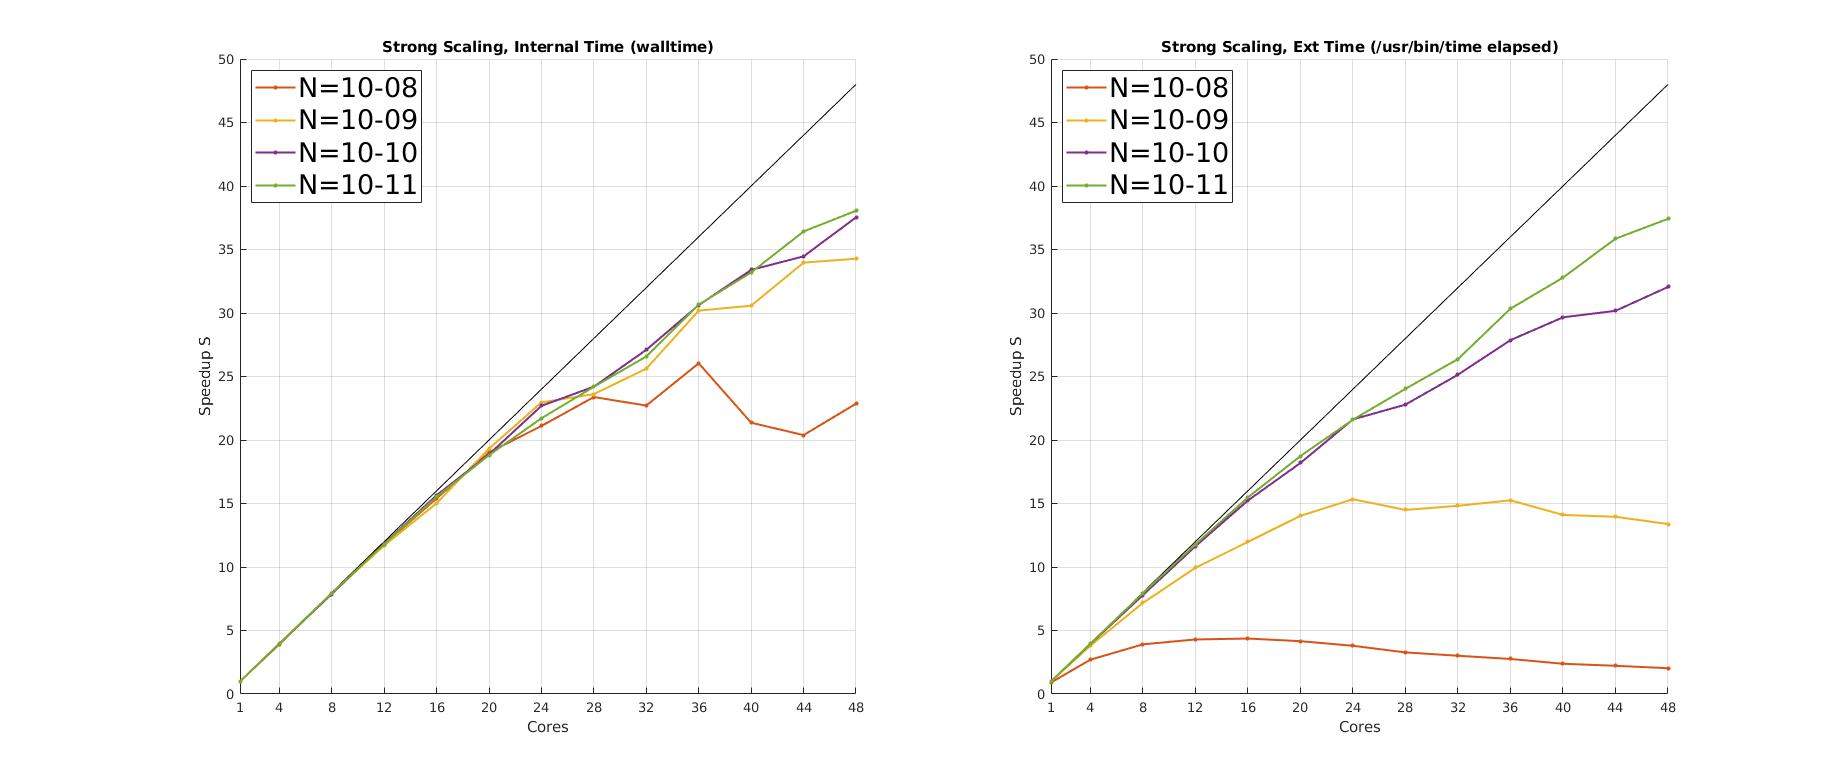
\includegraphics[width=1\textwidth]{strong_scaling2_noerror}
\caption{Direct comparison of scaling vs. $c$ curves for the four runs. Left panel is generated using internal time measurements, the right panel uses external times.}
\end{figure}
\label{strong_scaling2}
\end{center}																		
An attempt was made to build a model of the speedup curves for these strong-scaling tests. The goal was to extract coefficients that could capture the dependency of the parallel overheads on the number of processors.\\
Following, on the left side, are the proposed parallel run-time formulas for both the internally and externally-measured times, which lead to models for the internal and external speedup curves on the right:





\begin{minipage}{0.5\linewidth}
\begin{equation*}
\begin{split}
T_p^{int} \left( N, c \right) &= p \times \frac{N}{c} + k_1 \times \left( c - 1 \right) \\
T_p^{ext} \left( N, c \right) &= p \times \frac{N}{c} + k_1 \times \left( c - 1 \right) + k_2 \times c 
\end{split}
\end{equation*}
\end{minipage}
\begin{minipage}{0.5\linewidth}
\begin{equation}\label{speedup_model}
\begin{split}
S^{int} \left( N, c \right) &= \frac{T_s}{T_p^{int}} =  \frac{p\times N}{p \times \frac{N}{c} + k_1 \times \left( c - 1 \right)} \\
S^{ext} \left( N, c \right) &= \frac{T_s}{T_p^{ext}} = \frac{p\times N}{p \times \frac{N}{c} + k_1 \times \left( c - 1 \right) + k_2 \times c} 
\end{split}
\end{equation}
\end{minipage}



Two overhead coefficients $k_{1,2}$ are introduced. The fittings were conducted separately for each value of $N$ but simultaneously for the internal and external speedup curves. The coefficient $p$ was not treated as a fitting parameter, instead the value from Table \ref{serial_coefs} was re-used. Table \ref{speedup_fit_coefs} reports the fitting coefficients whie Figure \ref{strong_scaling_fits} overlays the fitting curves on top of the data already presented.


\begin{center}
 \begin{tabular}{|l | c | c | } 
 \hline
 $N$ & $ k_1 $  & $k_2$ \\ 
 \hline
 \hline
 $10^{8}$ & $0.001209 \pm 0.000070 $  & $ 0.02576 \pm 0.00422$\\
 \hline
 $10^{9}$ &  $0.004650 \pm 0.000175 $  & $ 0.02472 \pm 0.00081 $\\
 \hline
 $10^{10}$ &  $0.03590 \pm 0.00130 $   & $ 0.02489 \pm 0.00208$\\
 \hline
 $10^{11}$ &  $0.3335 \pm 0.0192$ & $ 0.02624 \pm 0.02688$\\
 \hline
\end{tabular}
\captionof{table}{Fitting coefficients for our theoretical speedup model for various values of $N$. }
\label{speedup_fit_coefs}
\end{center}


\begin{figure}[H]
\centering
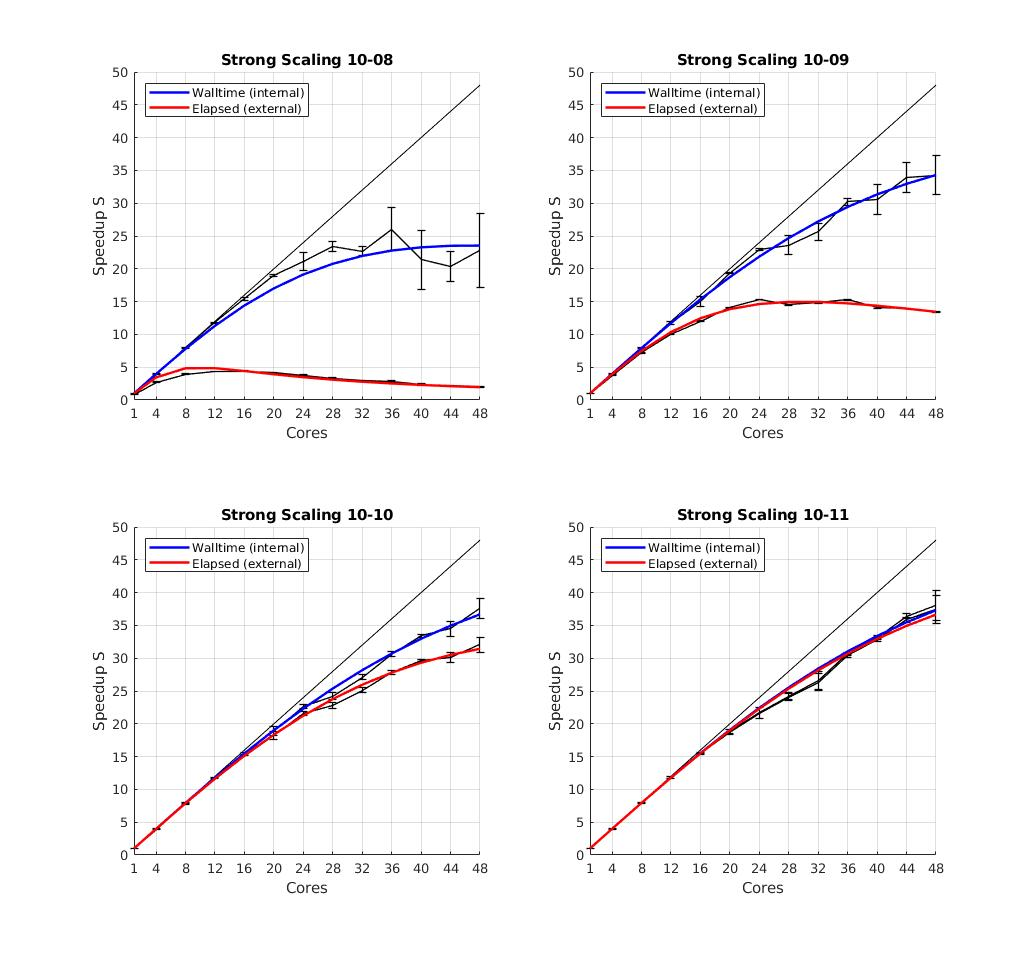
\includegraphics[width=0.85\textwidth]{strong_scaling_fits}
\caption{ Fit curves for the strong-scaling speedup. The curves are overlaid on top of the data curves (black). }
\label{strong_scaling_fits}
\end{figure}

The fitting curves capture the data trends reasonably well, although less so for the internal-time curve for $N=10^{8}$. Looking at the coefficients we notice that the values of $k_2$ are quite close to each other for all $N$, indicating that the \verb|MPI| initialisation overhead is the same across the different runs which is expected, as intiialising the framework for a processor should only depend on the computing environment and not on the problem size.
The error on $k_2$ for $N=10^{11}$ is however very large, this could indicate that the relative impact of the overhead for this size is so small that altering the coefficient significantly does not make much difference.\\
The $k_1$ coefficients, which model the communication overhead encompassed by the internal walltime, vary across the runs, suggesting once again that this overhead also depends on the problem size in some way.



\begin{minipage}{\linewidth}
\begin{minipage}{0.4\linewidth}
To gain insight on the dependency of $k_1$ on $N$ we plotted the four values on a semi-log graph, visible in figure \ref{k1_fit}. The coefficients seem to folow a linear trend, which was fitted with a linear relationship:


\begin{center}

\begin{equation}
k_1 \left( N \right) = c_1 + c_2\times N	
\end{equation}


 \begin{tabular}{|c | c | } 
 \hline
 $c_1$ & $ 0.001601  $  \\ 
 \hline
 $c_2$ & $ 0.3320\times 10^{-11} $ \\
 \hline
\end{tabular}
\captionof{table}{$k_1$ fit coefficients}
\label{serial_coefs}

\end{center}

Obviously the angular coefficient is very small, since the values of $N$ are so large, but nevertheless this is good evidence for the fact that the communication overhead carries linear ependency on $N$ itself.\\
It could be due to the fact that the master process collects results from the slaves in a very precise order and therefore, due to the nature of the synchronous send function, need to wait until both parties are ready. This wait time should depend on the sike of thework done by each processor which of course depends directly on $N$.

\end{minipage}
\begin{minipage}{0.6\linewidth}
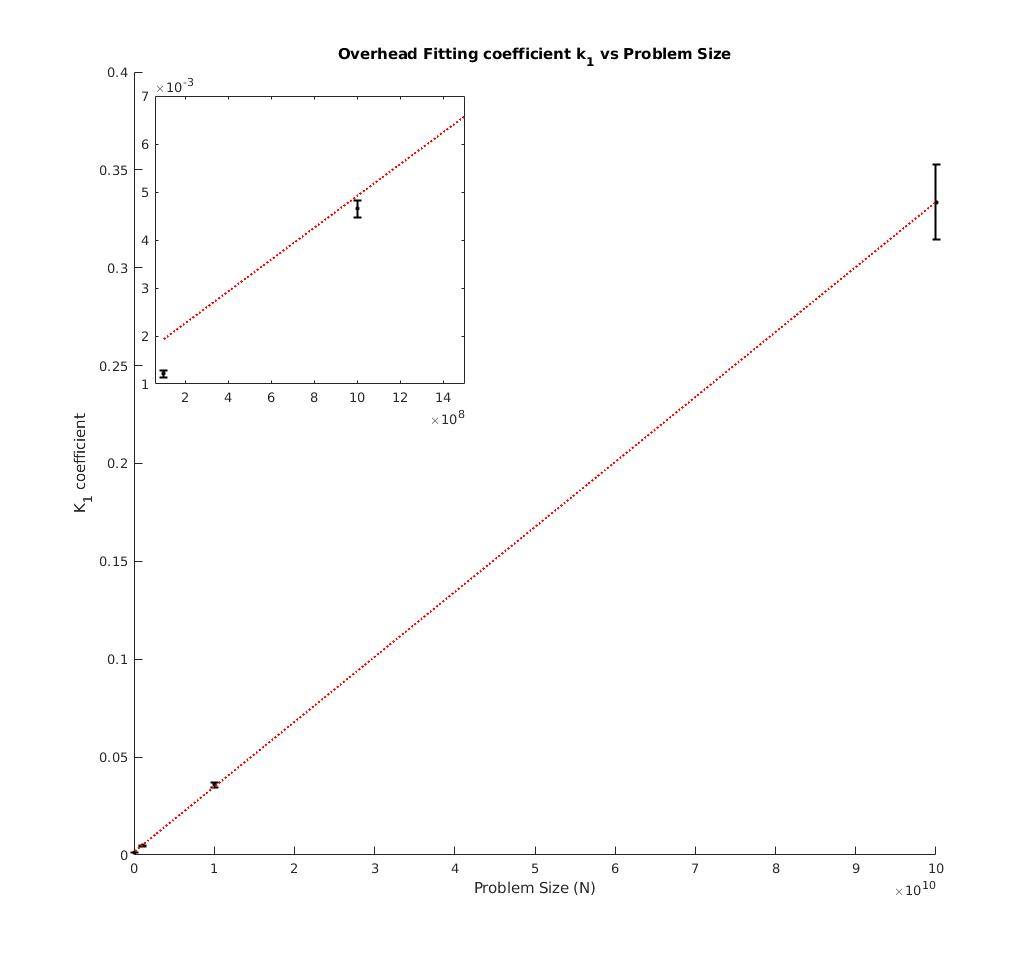
\includegraphics[width=0.8\textwidth]{k1_fit}
\captionof{figure}{Plot of the values of the $k_1$ fitting coefficient vs. problem size $N$, with a zoom on the lower-left quadrant. The dashed line represents a linear fitting curve. }
\label{k1_fit}
\end{minipage}
\end{minipage}




\subsection{Overhead Function Model}

In this section we construct a theoretical model for the so-calle \textit{Overhead function}, defined for a parallel algorithm as the total time spent by all processors to perform work that the best serial analogue program wouldn't do.\\
The total collective runtime of the parallel algorithm is $c \times T_p\left( c \right)$, which leads to the following:

\begin{equation}\label{overhead_def}
c  T_p\left( c \right) = T_s + T_o\left( c \right) \quad \Rightarrow \quad \frac{T_o\left( c \right)}{cT_p\left( c \right)} = 1 - \frac{T_s}{cT_p\left( c \right) }
\end{equation} 

where we wrote the ratio of the overhead function to the total parallel time, to be able to compare wildly different total run-times. The overhead fraction so defined is exactly complementary to the \textit{Efficiency} $S/c$, which is the fraction of time spend doing part of the serial work.\\
It is easy to build a theoretical model for this relative overhead, by writing the serial time in terms of the strong speedup $S$ and the parallel time and re-utilising the model built in equation \ref{speedup_model}:

\begin{minipage}{0.5\linewidth}
\begin{equation*}
\begin{split}
\frac{T_o\left( c \right)}{cT_p\left( c \right)}& = 1 - \frac{T_s}{cT_p\left( c \right) } = 1 - \frac{S\left( N, c \right)}{c} \\
S \left( N, c \right) &=\frac{p\times N}{p \times \frac{N}{c} + k_1 \times \left( c - 1 \right) + k_2 \times c}  \\
&= \frac{1}{ \displaystyle \frac{1}{c} + \frac{\left( k_1  + k_2\right)\times c -  k_1 }{p\times N} } 
\end{split}
\end{equation*}
\end{minipage}
\begin{minipage}{0.5\linewidth}
\begin{equation}\label{overhead_model}
\begin{split}
\frac{T_o\left( c \right)}{cT_p\left( c \right)}& = 1 - \frac{1}{ \displaystyle 1 + \frac{c \left( \left( k_1  + k_2\right)\times c -  k_1 \right)}{p\times N}  }
\end{split}
\end{equation}
\end{minipage}

The data curves for the total relative overhead was constructed using equation \ref{overhead_def} as a formula and using the externally-measured parallel times, and are plotted in figure \ref{overhead}. Figure \ref{overhead_fit} displays the theoretical models defined above for all values of $N$ and plugging the relative coefficients $p,k_1,k_2$.


\begin{figure}[H]
  \begin{subfigure}[h]{0.5\textwidth}
    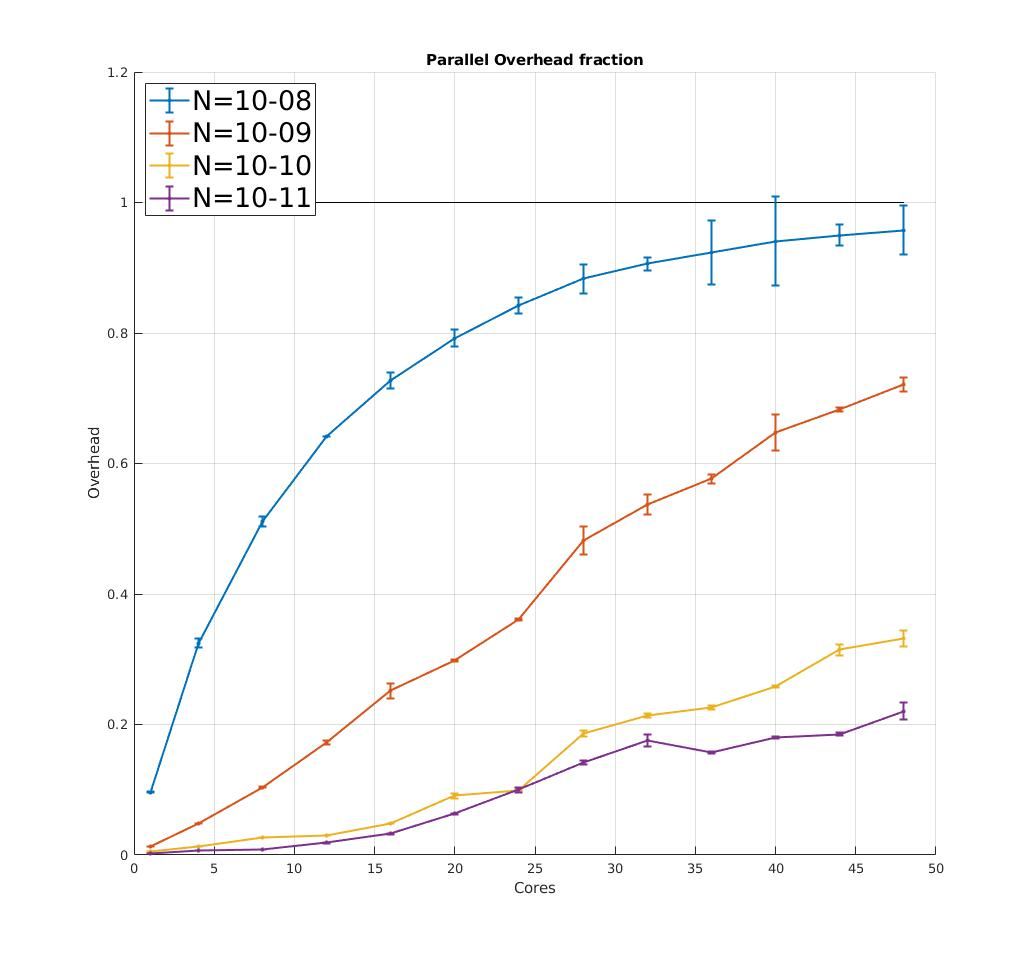
\includegraphics[width=\textwidth]{overhead}
    \caption{}
    \label{overhead}
  \end{subfigure}
  %
  \begin{subfigure}[h]{0.5\textwidth}
    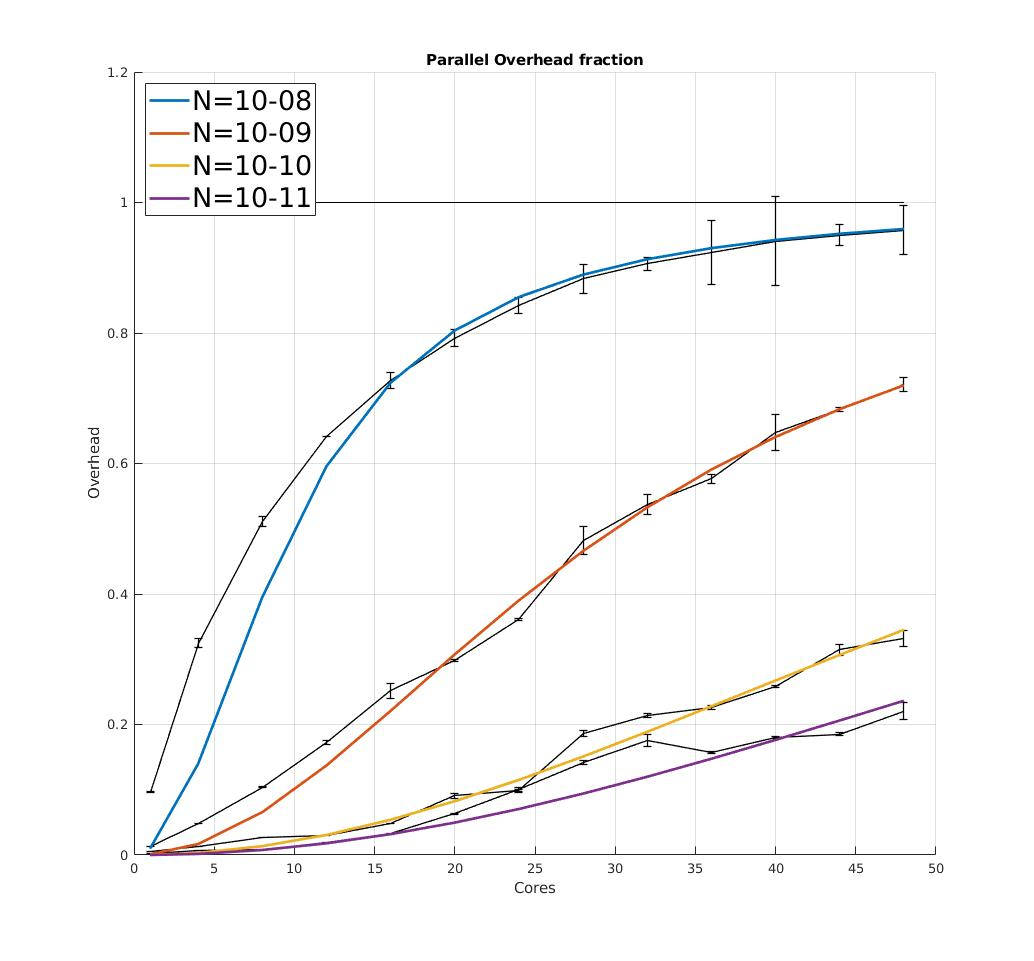
\includegraphics[width=\textwidth]{overhead_fit}
    \caption{}
    \label{overhead_fit}
  \end{subfigure}
   \caption{On the left: Total parallel overhead curves relative to total parallel time for various values of $N$. On the right: Fits of the total parallel overhead curves relative to total parallel time.  The curves are overlaid on top of the data curves (black).}
   \label{overhead_figs}
\end{figure}

Analysing the data plots, it is evident how the fraction becomes smaller as the problem size grows since the processors spend relatively more time doing "useful" work (useful towards the solution of the problem). All curves start close to zero when $c=1$ and grow as the number of processes increases, as expected. For the smallest problem size the fraction grows quickly and reaches almost 100\%, while the other curves grow more slowly since the larger problem size can better absorb the effects of the overheads.\\
Out fitting curves capture the trends rather well, in particular they all meet at $c=1$, where the overhead is exactly zero. The fitting is quite good for large values of $c$, while it is poorer for the smaller values.

\subsection{Weak Scaling}

We move on to studying the \texttt{Weak scaling} of the parallel algorithm. That is, starting from a problem of size $N$ assigned to a single worker, as more processors $c$ are added the problem size is increased by the same factor: $c \times N$.\\
Similarly to the strong scaling, four reference values of the problem size $N=\left\{ 10^{8}, 10^{9}, 10^{10}, 10^{11} \right\}$ were considered along with varying number of workers $c=\left\{ 1, 4, 8, 12, \dots , 48 \right\}$.
For each combination of $\left(c,N\right)$ three runs were performed, the average runtimes and their error bars are plotted for the four values of $N$ in Figure \ref{weak_runtimes}.


\begin{figure}[H]
\centering
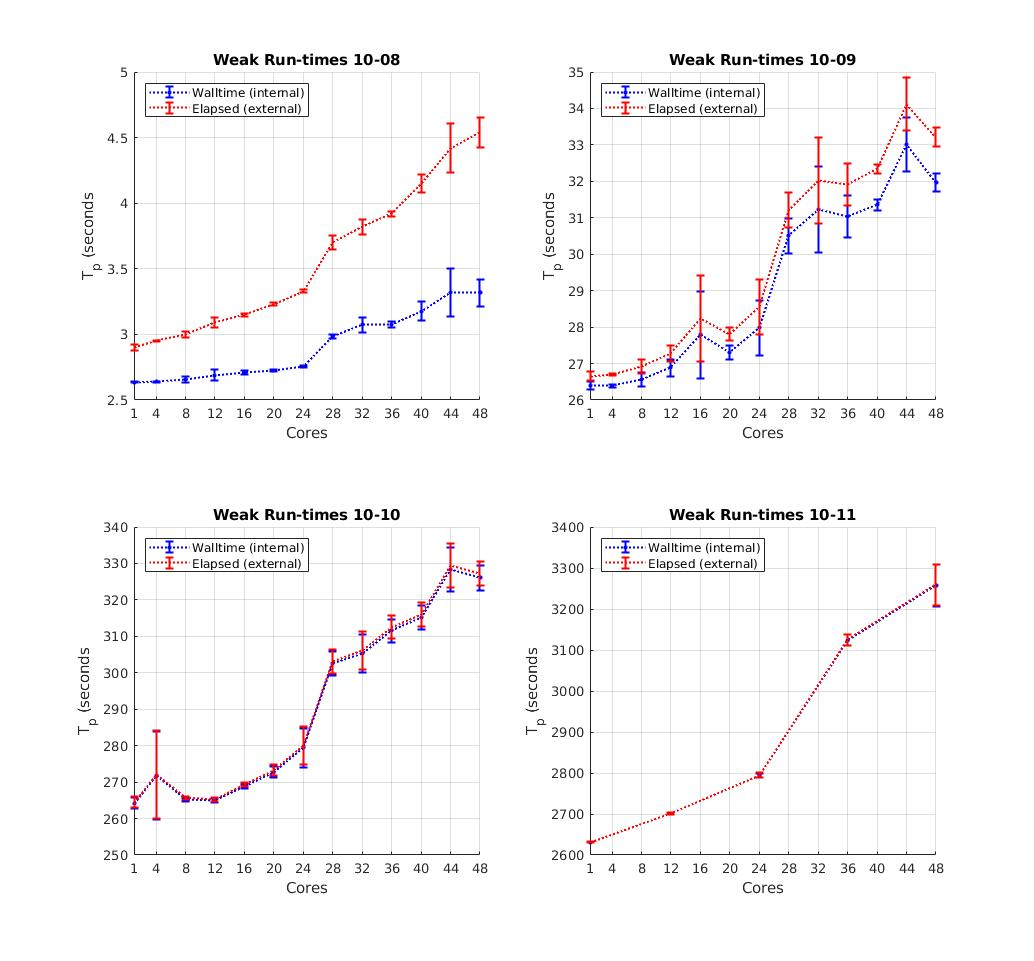
\includegraphics[width=0.85\textwidth]{weak_runtimes}
\caption{WEak-scaling runtimes against the number of processors $c$ for different values of the problem size $N$. Blue curves represent the "walltime" internal to the program, while the red curves use the externally measured run-time}
\label{weak_runtimes}
\end{figure}

While ideal strong scaling of the problem would imply that $c$ workers can do the same work in a time $\propto 1/c$, ideal weak scaling would predict that the run-time stays constant as the work done  per processor stays constant. As we proced experimentally, strong scaling is impaired by the parallel overheads which add more work as both the problem size $N$ and the number of workers $c$ increases. We also expect the weak scaling to suffer from a similar issue, although we can expect better scaling properties since the ever larger problem size entails that the parallel overheads become less important compared to the "useful" work time. This is essentially the same behaviour found for the strong scaling case when comparing different $N$ values.
\par 
To assess the weak scaling performance we consider the weak-scaling efficiency $E = T \left( 1 \right) / T_p \left( c \right) $ where $T \left( 1 \right)$ refers still to the best serial algorithm for the problem of size $N$ and $T_p \left( c \right)$ is the parallel run-time for a problem of size $c\times N$ over $c$ workers. Figure \ref{weak_scaling1} reports the weak efficiency curves for various reference values of $N$.\\
The blue internal-time curves show the downwards trend in efficiency as $c$ increases, and it is interesting to note that the curves all look very similar to each other (evident in the left panel of figure \ref{weak_scaling2}). This indicates that the weak scaling does not depend on the absolute value of $N$ and is instead influenced by the overheads. The red curves display the ful effect of the overheads, which has a heavy impact on eficiency for the smallest value of $N$ and are progressively less important as the reference $N$ grows. This is because the intialisation overhead depends on $c$ but not $N$.\\
The efficiency in the strong scaling case may be deduced as the complementary of the Overhead function represented in figure \ref{overhead}, comparing this with the weak efficiency curves it can be seen how this algorithm scales better in the weak sense rather than the strong sense: for the highest value of $c$ the weak efficiency values are all between about 60-80\%, compared to strong efficiencies of less than 10\% for the smallest problem size.

\begin{figure}[H]
\centering
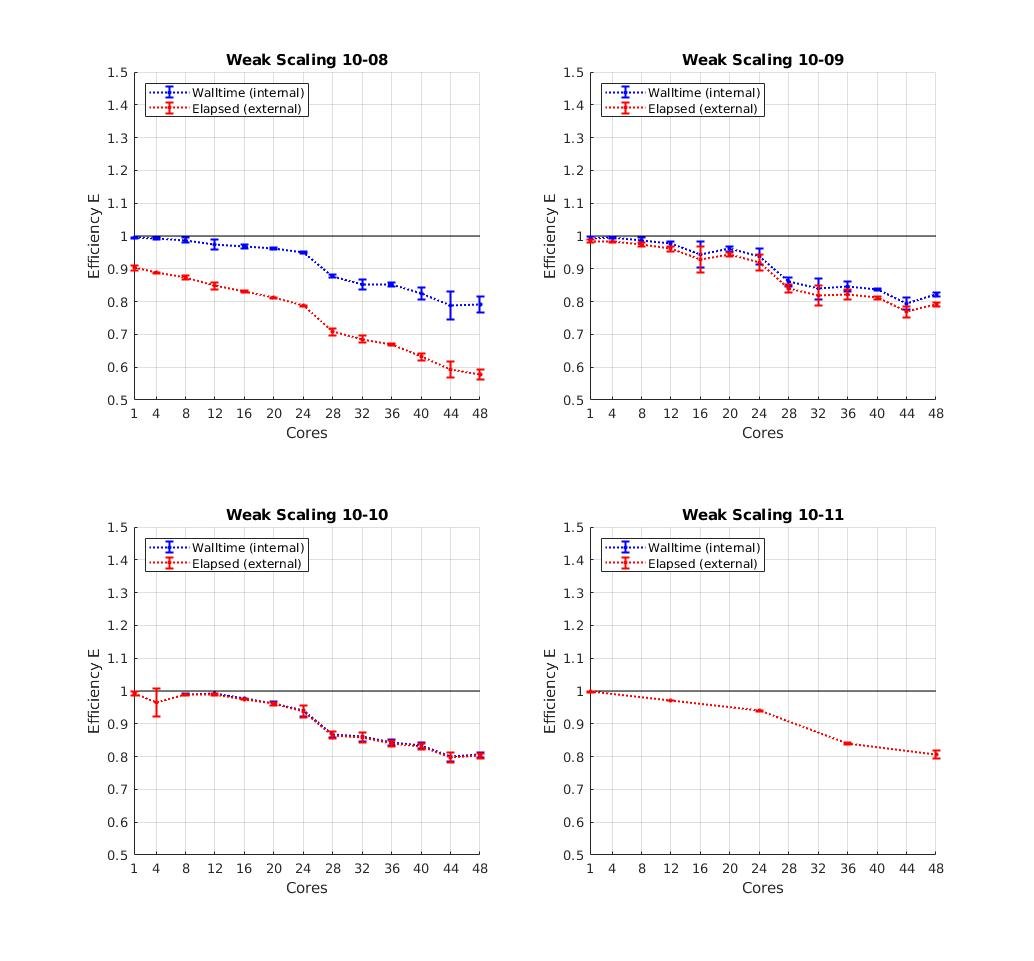
\includegraphics[width=0.8\textwidth]{weak_scaling1}
\caption{Weak Efficiency curves for the parallel algorithm against the number of processors $c$ for different reference values of the problem size $N$. Blue curves represent the "walltime" internal to the program, while the red curves use the externally measured run-time. }
\label{weak_scaling1}
\end{figure}

\begin{figure}[h]
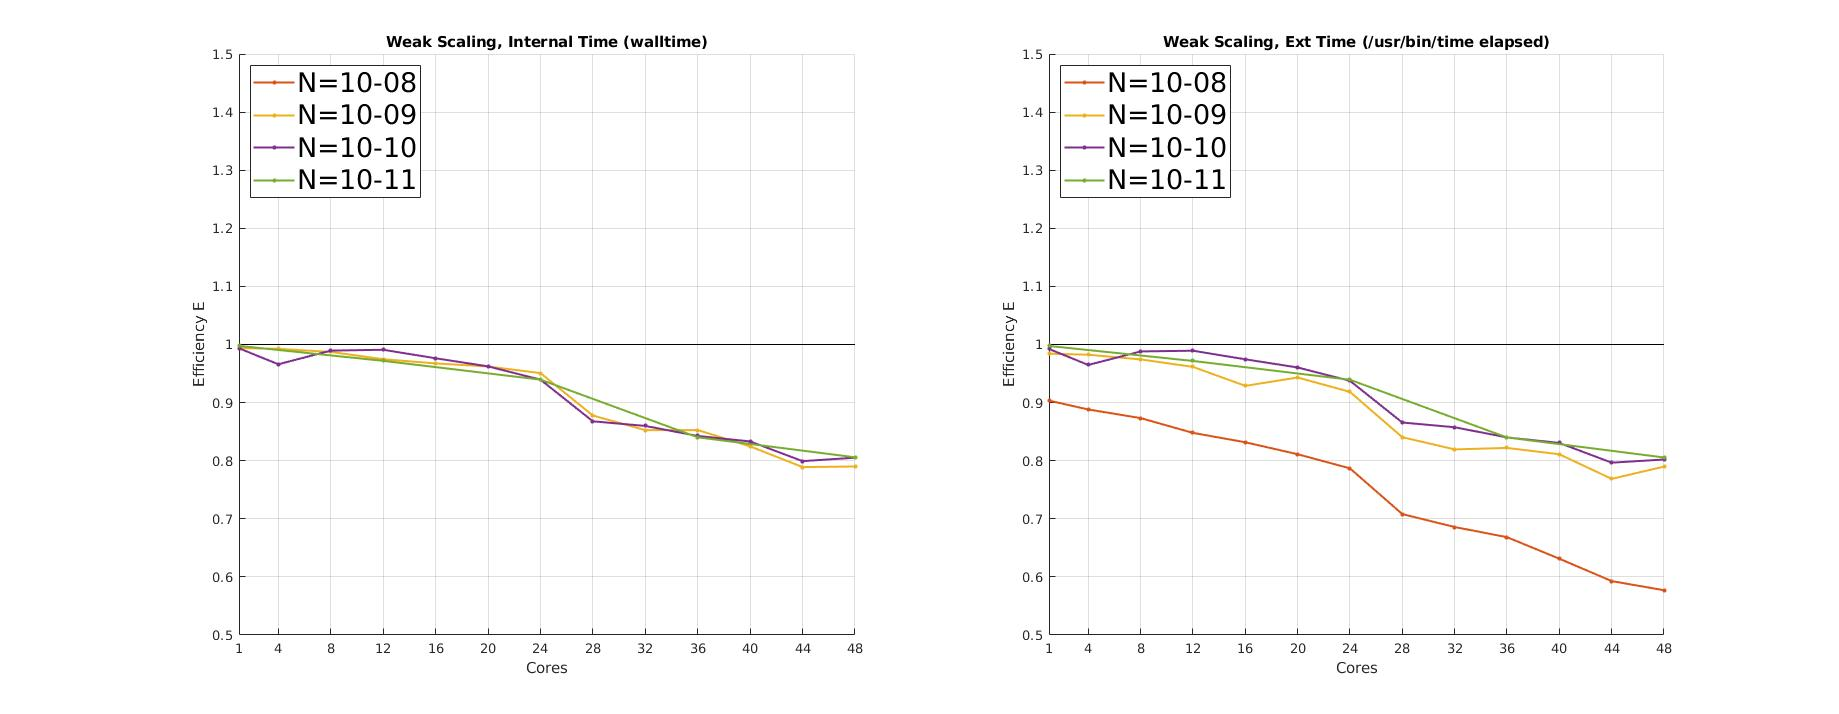
\includegraphics[width=0.9\textwidth]{weak_scaling2}
\caption{Direct comparison of weak efficiency vs. $c$ curves for the four runs. Left panel is generated using internal time measurements, the right panel uses external times.}
\end{figure}
\label{weak_scaling2}


To model the weak efficiency, the toy models for the parallel run-times were re-cycled from equation \ref{speedup_model}, with modifications to account for the growth of the problem size with $c$:

\begin{minipage}{0.5\linewidth}
\begin{equation*}
\begin{split}
T_p^{int} \left( N, c \right) &= p N + k_1 \left( c - 1 \right) c \\
T_p^{ext} \left( N, c \right) &= p N + k_1 \left( c - 1 \right)c + k_2 c 
\end{split}
\end{equation*}
\end{minipage}
\begin{minipage}{0.5\linewidth}
\begin{equation}\label{weak_eff_model}
\begin{split}
E^{int} \left( N, c \right) &= \frac{p N}{p N + k_1 \left( c - 1 \right) c} \\
E^{ext} \left( N, c \right) &= \frac{p N}{p N + k_1 \left( c - 1 \right)c + k_2 c } 
\end{split}
\end{equation}
\end{minipage}

The $k_1$ terms are multiplied by an additional factor $c$ since it was previously determined that the associated overhead carries linear dependency on the problem size. The previous coefficients of Table \ref{speedup_fit_coefs} were re-used in thos theoretical model, the resulting curves are plotted against the data in figure \ref{weak_scaling_fit}.


\begin{figure}[H]
\centering
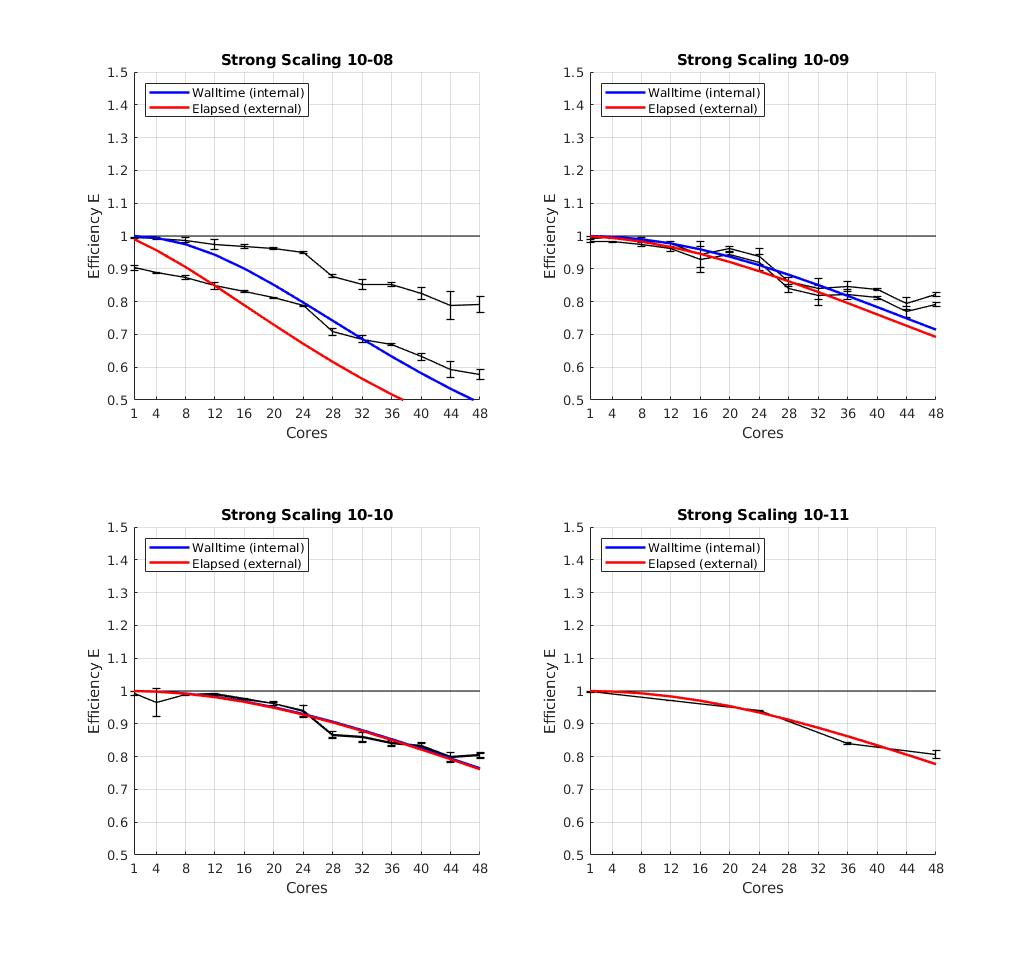
\includegraphics[width=0.85\textwidth]{weak_scaling_fit}
\caption{Weak Efficiency fitting curves for the parallel algorithm against the number of processors $c$ for different reference values of the problem size $N$. Blue curves represent the "walltime" internal to the program, while the red curves use the externally measured run-time.  }
\label{weak_scaling_fit}
\end{figure}

The model is quite good for large reference values of $N$ and very poor for the smaller values, in that the weak efficiency scales better than predicted. The model accurately predicts the trend when the overheads have the least importance relative to the problem size, so the issue could be due to over-estimation of the overhead coefficients, which were re-utilised from the strong scaling.

\section{Conclusions}

In the first section, two simple theoretical models for the run-time of a  parallel algorithm dealing with the summation of $N$ numbers was formulated, the main features of Amdahl's law were confirmed, regarding the presence of a non-parallelisable fraction of the program as well as the effect of the various overheads induced by the parallelisation. The performance gains of processor communication methods which can take advantage of parallelisation were also demonstrated.\\
In the second section, the performance of a parallel algorithm for the calculation of $\pi$ was studied, both in strong and weak scaling. The algorithm was seen to have a large degree of parallelisation, i.e. a very small serial fraction, but substantial overheads given both by inter-processor communication and \verb|MPI|-environment initialisation. For the strong scaling tests, the expected trends given by Amdahl's law were noticed. A simple theoretical model was constructed for the strong Speedup curves which suggested that the intialisation overhead depends exclusively on the numebr of workers involved, while the communication overhead depends also on the problem size. This model was naturally extended to the overhead function with good results.\\
The weak scaling performance was asessed, and it was seen that this algorithm is able to maintain good weak efficiency across the entire range of number of processors studied, contrary to what was seen for the strong scaling. This is evidnce that the weak scaling operation is a good way to moderate the impact of parallel overheads. Our theoretical toy model was adapted to represent weak efficiency with mixed results, possibly due to the re-cycling of fitting coefficents which constitute overestimates of the overheads especially for the smallest problem size runs.

%----------------------------------------------------------------------------------------
%	BIBLIOGRAPHY
%----------------------------------------------------------------------------------------

%\bibliographystyle{unsrt}

%\bibliography{report_bib}

%----------------------------------------------------------------------------------------


\end{document}